\documentclass[10pt]{article}
\usepackage[margin=0.72in,top=0.65in,bottom=0.65in]{geometry}
\usepackage[T1]{fontenc}
\usepackage[utf8]{inputenc}
\usepackage{lmodern}
\usepackage{setspace}
\usepackage{graphicx}
\usepackage{hyperref}
\usepackage{float}
\usepackage{caption}
\usepackage{microtype}
\usepackage{listings}
\usepackage{xcolor}
\usepackage{enumitem}

\graphicspath{{assets/}}
\setstretch{1.0}
\tolerance=400
\emergencystretch=1em
\setlength{\parskip}{2pt plus 1pt}
\setlength{\parindent}{0.8em}
\hypersetup{colorlinks=true,linkcolor=black,urlcolor=blue}
\captionsetup{font=small,labelfont=bf,skip=4pt}

\lstset{
  basicstyle=\ttfamily\scriptsize,
  keywordstyle=\bfseries,
  commentstyle=\color{gray},
  breaklines=true,
  frame=single,
  framesep=3pt,
  xleftmargin=4pt,
  xrightmargin=4pt,
  aboveskip=4pt,
  belowskip=4pt,
}

\title{\vspace{-1.5em}Task 3 -- Data Model and Application Design: MongoDB + AirBnB\vspace{-0.5em}}
\author{Abhinav Bachu, Hanshul Bahl, Alejandra Arias\\CS 498 / Data Management in the Cloud}
\date{04/01/2026}

\begin{document}
\maketitle
\vspace{-1.8em}

%% ========== SECTION 1 ==========
\section{Selected Storage System and Dataset}

We're using \textbf{MongoDB} as our storage system and the \textbf{InsideAirbnb} dataset as our project dataset. The data covers four cities---Los Angeles, Portland, Salem, and San Diego---and comes in four file types per city: \texttt{listings.csv.gz} (detailed listing metadata), \texttt{calendar.csv.gz} (day-level availability and pricing), \texttt{reviews.csv.gz} (individual review events with reviewer identifiers), and \texttt{neighbourhoods.csv} (canonical neighborhood names). Across the four cities the raw data totals about 1.4\,GB.

For this milestone we designed for the full query scope but loaded a representative subset for proof of concept. Everything in this report---collections, indexes, query strategies---is built against the real schema and column names from the full dataset; we just cap the row count so ingestion stays fast while we iterate on the design. The subset covers all four cities and all four entity types, which is enough to verify that document shapes, indexes, and aggregation pipelines behave as expected before scaling up in Part~3.


%% ========== SECTION 2 ==========
\section{Data Representation in MongoDB}

\subsection{Final Representation}

The final design uses four collections: \texttt{listings}, \texttt{calendar}, \texttt{reviews}, and \texttt{neighborhoods}. Each source file maps to its own collection, and every document carries a \texttt{city} field so that multi-city queries can filter without needing separate databases.

The main modeling question was whether to embed calendar and review data inside listing documents or keep them in separate collections. Embedding has some appeal since it puts everything about a listing in one read, but it doesn't hold up well for this dataset. Calendar has one row per listing per day for an entire year, which means a single listing document would contain 365 or more embedded subdocuments. Reviews accumulate over years and grow without a fixed bound. In practice that combination makes documents large, rewrites costly, and indexing harder for the time-window and trend queries the assignment calls for.

With separate collections, \texttt{listings} holds the expected metadata---name, neighborhood, room type, property type, accommodates, price, host identifiers, review scores, URL, description, and amenities. \texttt{calendar} holds day-level availability as a boolean flag along with per-night pricing and minimum/maximum night constraints. \texttt{reviews} holds the reviewer ID, reviewer name, date, and comment text. \texttt{neighborhoods} is basically a lookup table of city--neighborhood pairs, which exists mainly for the completeness check in Query~2. This split lines up well with the six assignment queries, which involve a mix of listing lookups, date-range filtering, monthly aggregation, and repeated-reviewer logic.

\begin{figure}[t]
\centering
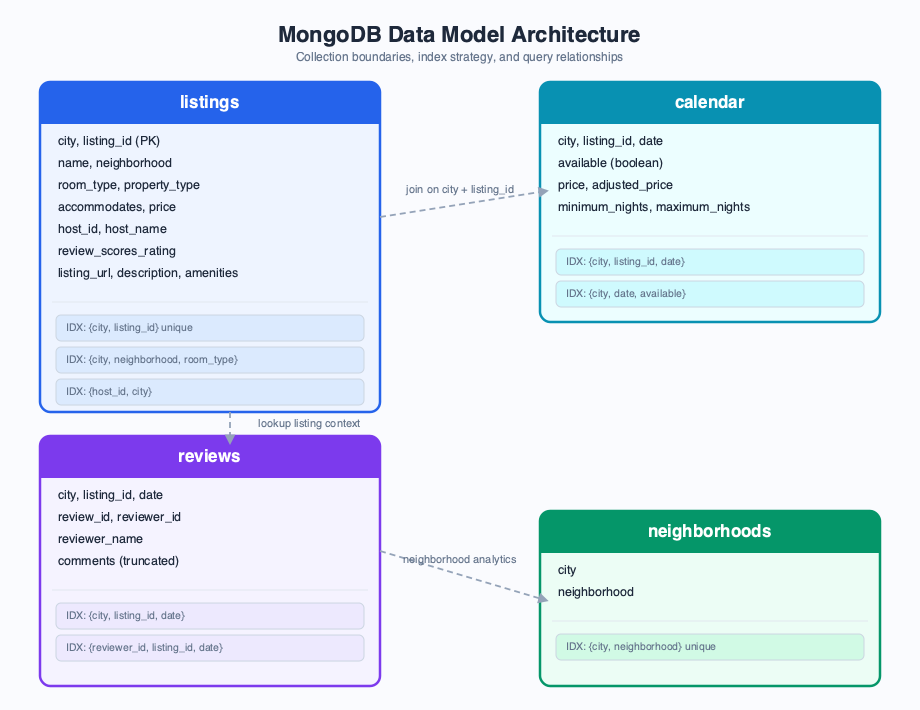
\includegraphics[width=0.88\textwidth]{model_diagram_python.png}
\caption{Data model architecture: four MongoDB collections, key fields, compound indexes, and query relationships.}
\label{fig:model}
\end{figure}

\subsection{Indexes}

The index strategy follows from the six query patterns. We use \texttt{\{city, listing\_id\}} as the unique key in \texttt{listings}, since nearly every query starts by isolating a city and then joining on listing ID. A compound index on \texttt{\{city, neighborhood, room\_type\}} covers queries that filter by location and type, and \texttt{\{host\_id, city\}} supports Query~6's same-host expansion.

On the \texttt{calendar} side, \texttt{\{city, listing\_id, date\}} handles per-listing date-range lookups and
\texttt{\{city, date, available\}} handles city-wide availability filtering. For \texttt{reviews},
\texttt{\{city, listing\_id, date\}} covers monthly review counts, and a second index on
\texttt{\{reviewer\_id, listing\_id, date\}} supports the repeated-reviewer detection in Query~6. \texttt{neighborhoods} gets a unique index on \texttt{\{city, neighborhood\}}. We didn't add any speculative indexes beyond these, since each one has a cost on writes and we'd rather validate with \texttt{explain()} in Part~3 and add more only if we need them.

\subsection{Alternative Representation Considered}

We also considered a fully denormalized approach where each listing document embeds its entire calendar array and reviews array. That eliminates the \texttt{\$lookup} for some per-listing reads, but calendar data is large and changes frequently, which means embedded documents get rewritten often and can approach MongoDB's 16\,MB document limit. Running \texttt{\$unwind} over large embedded arrays also gets expensive for city-wide monthly analytics, and it removes the ability to put targeted compound indexes on date ranges the way a standalone \texttt{calendar} collection allows. Since most of the six queries involve time-window filtering or city-level aggregation, the multi-collection design ended up being a better fit.


%% ========== SECTION 3 ==========
\section{Restructuring, Cleaning, and Loading Process}

The raw files require some cleaning before they can be loaded. City names are normalized to lowercase keys (\texttt{los\_angeles}, \texttt{portland}, \texttt{salem}, \texttt{san\_diego}) so that multi-city queries can filter on a single consistent field. Numeric columns like \texttt{price} and \texttt{minimum\_nights} come in as strings with dollar signs and commas, so those are parsed into actual numbers. The \texttt{available} column uses \texttt{t}/\texttt{f} strings, which we convert to booleans. Dates are preserved as ISO strings for now; we handle \texttt{Date} conversion at query time where date arithmetic is needed.

We only keep the fields that the six queries actually use, and drop everything else to keep documents small. Records that are missing a listing ID or have a malformed date are discarded, and description and comment text is truncated to 200 characters since none of the queries need the full content.

The loading is handled by a script (\texttt{scripts/load\_and\_capture.js}) that fetches data from all four cities, cleans and reshapes each row into collection-specific document shapes, inserts via \texttt{insertMany()}, creates all the compound indexes, and writes an evidence transcript with collection counts, sample documents, and index metadata. The script runs on \texttt{mongodb-memory-server}, so it doesn't require a persistent MongoDB deployment to reproduce.

\begin{figure}[t]
\centering
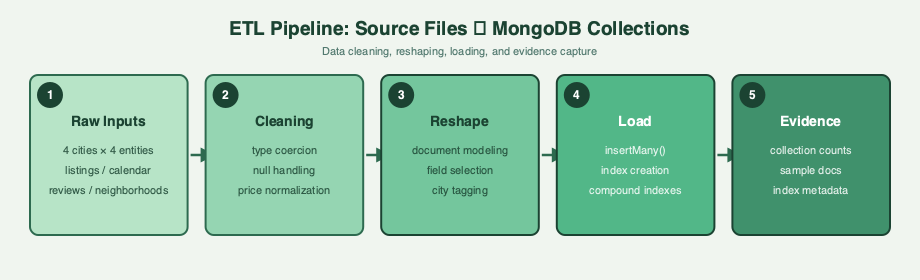
\includegraphics[width=0.88\textwidth]{etl_diagram_python.png}
\caption{ETL workflow from raw CSV files through cleaning, reshaping, loading, and evidence capture.}
\label{fig:etl}
\end{figure}


%% ========== SECTION 4 ==========
\section{Query Implementation Strategies (Pseudocode)}

The pseudocode below covers all six queries, written against the MongoDB aggregation framework and the indexes described above. Each strategy notes which collections and indexes it relies on.

\subsection{Query 1: Portland Search for a Two-Day Window}

Display Portland listings available on both days of a requested two-day period, with details, sorted by average rating descending.

\begin{lstlisting}
// Indexes: calendar {city,listing_id,date}, listings {city,listing_id}
// Step 1: find listing_ids available on BOTH days
candidates = db.calendar.aggregate([
  { $match: { city:"portland", date:{$in:[day1,day2]}, available:true }},
  { $group: { _id:"$listing_id", days:{$sum:1} }},
  { $match: { days: 2 }}
])
// Step 2: join to listings, project fields, sort by rating
db.listings.aggregate([
  { $match: { city:"portland", listing_id:{$in: candidates._id} }},
  { $project: { _id:0, name:1, neighborhood:1, room_type:1, accommodates:1,
      property_type:1, amenities:1, price:1, review_scores_rating:1 }},
  { $sort: { review_scores_rating: -1 }}
])
\end{lstlisting}

\subsection{Query 2: Neighborhoods with No Listings in a Given Month}

For any city, find neighborhoods that have zero available listings during a target month.

\begin{lstlisting}
// Indexes: calendar {city,date,available}, neighborhoods {city,neighborhood}
// Step 1: derive active neighborhoods from calendar+listings join
activeNeighborhoods = db.calendar.aggregate([
  { $match: { date:{$gte:monthStart,$lte:monthEnd}, available:true }},
  { $group: { _id:{ city:"$city", lid:"$listing_id" }}},
  { $lookup: { from:"listings", let:{c:"$_id.city",l:"$_id.lid"},
      pipeline:[{$match:{$expr:{$and:[{$eq:["$city","$$c"]},
        {$eq:["$listing_id","$$l"]}]}}},{$project:{neighborhood:1}}],
      as:"info" }},
  { $unwind:"$info" },
  { $group: { _id:{ city:"$_id.city", neighborhood:"$info.neighborhood" }}}
])
// Step 2: anti-join -- collect active set, then exclude via $nin
activeSet = activeNeighborhoods.map(r => r._id)  // [{city,neighborhood},...]
for each city c in dataset:
  activeNames = activeSet.filter(a => a.city==c).map(a => a.neighborhood)
  db.neighborhoods.find({
    city: c,
    neighborhood: { $nin: activeNames }  // neighborhoods with zero listings
  })
\end{lstlisting}

\subsection{Query 3: Salem Entire-Home Availability Periods}

For each ``Entire home/apt'' listing in Salem, find the contiguous bookable windows within a target month, taking into account that minimum-night requirements can vary by day.

\begin{lstlisting}
// Indexes: listings {city,neighborhood,room_type}, calendar {city,listing_id,date}
ids = db.listings.find({ city:"salem", room_type:"Entire home/apt" },
  { listing_id:1, name:1 })
rows = db.calendar.find({ city:"salem", listing_id:{$in:ids},
  date:{$gte:monthStart,$lte:monthEnd} }).sort({ listing_id:1, date:1 })
// Application logic per listing:
//   a) scan consecutive available=true runs
//   b) keep day only if remaining_run_length >= minimum_nights(day)
//   c) merge valid days into [from, to] intervals
//   d) output: listing_name, month, from-to, min_nights
\end{lstlisting}

The consecutive-day validation here---checking each day's minimum-night constraint against how many days remain in the run---is awkward to express purely in aggregation. A hybrid approach (indexed fetch followed by application-side interval detection) is clearer and easier to test independently.

\subsection{Query 4: Portland Booking Trend March--August}

Total bookable nights per month for Portland ``Entire home/apt'' listings, reusing Query~3's interval logic.

\begin{lstlisting}
// Reuse interval computation from Query 3 in a loop
for each month in [March..August]:
  intervals = computeBookableIntervals("portland", "Entire home/apt", month)
  // intervals already exclude days where the remaining consecutive run
  // is shorter than that day's minimum_nights -- only surviving intervals
  // contribute to the monthly total
  totalNights[month] = sum(interval.to - interval.from + 1)
return [{ month, totalNights }, ...]
\end{lstlisting}

We keep the interval-detection logic in one shared function so that Queries~3 and 4 apply the same rules. A night counts toward the monthly total only if it belongs to a consecutive available run whose length meets or exceeds that day's minimum-night requirement for the listing; isolated available days that fall below the threshold are excluded.

\subsection{Query 5: Reviews in December by City and Year}

For each city, count how many reviews were received during December of each year.

\begin{lstlisting}
// Index: reviews {city, listing_id, date}
db.reviews.aggregate([
  { $addFields: { d: { $toDate: "$date" }}},
  { $match: { $expr: { $eq:[{$month:"$d"}, 12] }}},
  { $group: { _id:{ city:"$city", year:{$year:"$d"} }, count:{$sum:1} }},
  { $sort: { "_id.city":1, "_id.year":1 }}
])
\end{lstlisting}

\subsection{Query 6: Reminder to Book Again + Same-Host Expansion}

Find reviewer--listing pairs where the reviewer has left more than one review, check whether the listing is available in the same calendar month as a prior review, and include any other listings by the same host in the same city.

\begin{lstlisting}
// Indexes: reviews {reviewer_id,listing_id,date},
//   calendar {city,listing_id,date}, listings {host_id,city}
repeats = db.reviews.aggregate([
  { $addFields: { d:{$toDate:"$date"} }},
  { $group: { _id:{city:"$city", lid:"$listing_id", rid:"$reviewer_id"},
      dates:{$push:"$d"}, cnt:{$sum:1} }},
  { $match: { cnt:{$gt:1} }}
])
for (group of repeats):
  for (priorDate of group.dates):
    [mStart, mEnd] = monthBounds(priorDate)
    // Check if listing is available in that same month
    avail = db.calendar.findOne({ city:group._id.city,
      listing_id:group._id.lid, date:{$gte:mStart,$lte:mEnd}, available:true })
    listing = db.listings.findOne({ city, listing_id })
    // Expand to other listings by same host in same city
    others = db.listings.find({ city:listing.city, host_id:listing.host_id,
      listing_id:{$ne:listing.listing_id} })
    emit({ name, url, description, host_name, reviewer_name,
      previously_booked:true, month, min_nights, max_nights,
      available_in_same_month: avail!=null, other_host_listings: others })
\end{lstlisting}


%% ========== SECTION 5 ==========
\section{Screenshot Evidence of Loaded Data}

The screenshot below is from a live \texttt{mongosh} session run against the proof-of-concept database. It shows collection counts (200 listings, 320 reviews, 98 neighborhoods, 480 calendar rows across the four cities), sample documents from each collection, and the compound indexes.

\begin{figure}[H]
\centering
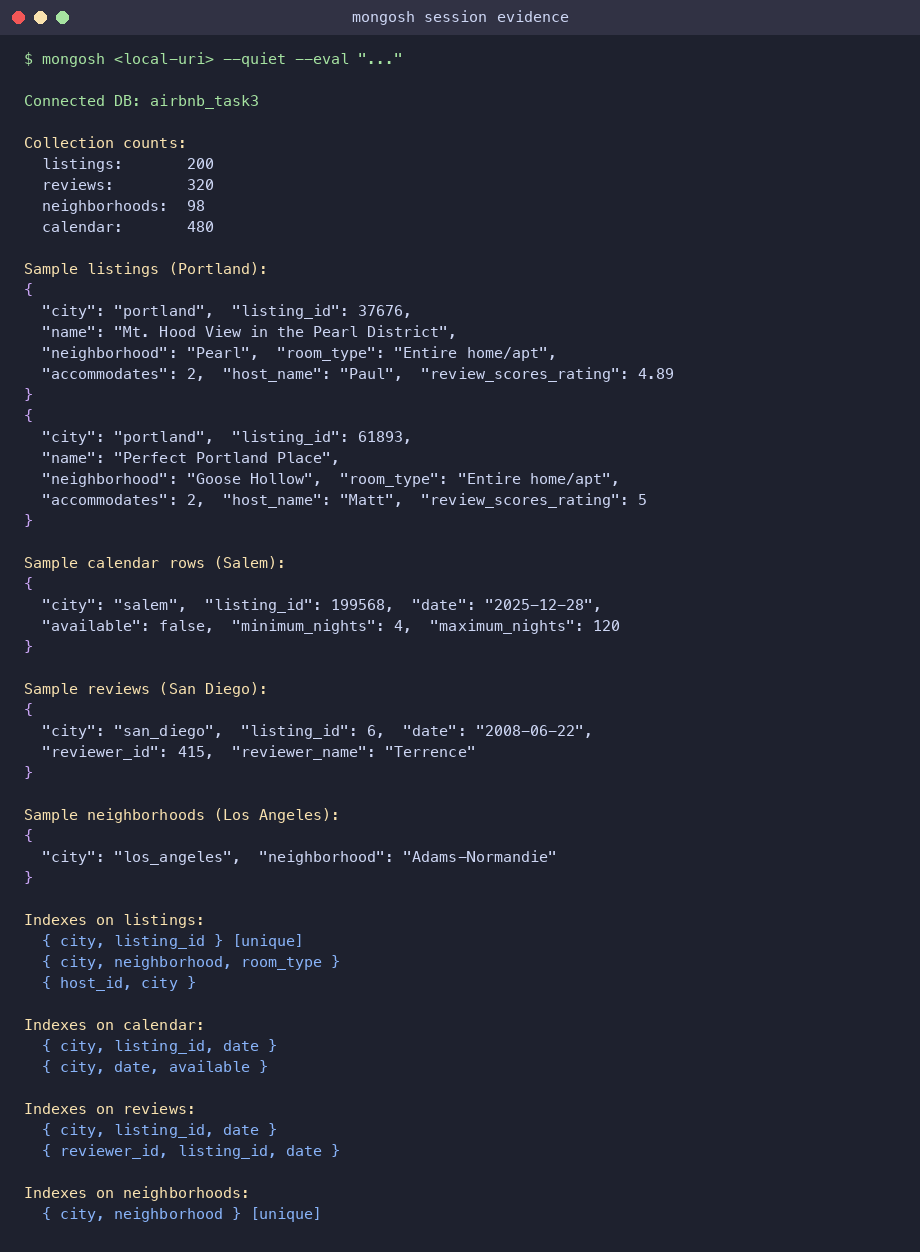
\includegraphics[width=0.72\textwidth,height=0.36\textheight,keepaspectratio]{mongosh_evidence_screenshot.png}
\caption{Live \texttt{mongosh} session: collection counts, sample documents, and index metadata.}
\label{fig:evidence}
\end{figure}


%% ========== SECTION 6 ==========
\section{Implementation Notes for Part 3 Readiness}

For Part~3, the most important decision is keeping the booking-window logic in a single reusable module. Queries~3 and 4 both depend on the same consecutive-availability and minimum-night checks, and having that code in one place avoids subtle divergence and makes it straightforward to unit-test without touching the database. Beyond that, we'll want to validate index effectiveness at full data scale using \texttt{explain()} and adjust field order if any query falls back to a collection scan. The collection split also leaves room to introduce a precomputed monthly-availability collection later if Queries~3--4 turn out to be slow at full size.

\clearpage
\section*{References}
\begin{enumerate}[leftmargin=*,label={[\arabic*]}]
\item MongoDB Documentation. \url{https://www.mongodb.com/docs/manual/}
\item MongoDB Aggregation Pipeline. \url{https://www.mongodb.com/docs/manual/core/aggregation-pipeline/}
\item MongoDB Indexes. \url{https://www.mongodb.com/docs/manual/indexes/}
\item MongoDB Data Modeling. \url{https://www.mongodb.com/docs/manual/core/data-model-design/}
\item MongoDB \texttt{\$lookup} Operator. \url{https://www.mongodb.com/docs/manual/reference/operator/aggregation/lookup/}
\item MongoDB Query Operators. \url{https://www.mongodb.com/docs/manual/reference/operator/query/}
\item InsideAirbnb Data Portal. \url{https://insideairbnb.com/get-the-data.html}
\end{enumerate}

\end{document}
